%%%%%%%%%%%%%%%%%%%%%%%%%%%%%%%%%%%%%%%%%%%%%%%%%%%%%%%%%%%%%%%%%%%%%%%%%%%%%%%%%%%%%%%%%%%%%%%%%%%%%%%%%%%%%%%%%%%%%%%%%%%%%%%%%%%%%%%%%%%%%%%%%%%%%%%%%%%%%%%%%%%
% Written By Michael Brodskiy
% Class: Embedded Design: Enabling Robotics
% Professor: S. Shazli
%%%%%%%%%%%%%%%%%%%%%%%%%%%%%%%%%%%%%%%%%%%%%%%%%%%%%%%%%%%%%%%%%%%%%%%%%%%%%%%%%%%%%%%%%%%%%%%%%%%%%%%%%%%%%%%%%%%%%%%%%%%%%%%%%%%%%%%%%%%%%%%%%%%%%%%%%%%%%%%%%%%

\documentclass[12pt]{article} 
\usepackage{alphalph}
\usepackage[utf8]{inputenc}
\usepackage[russian,english]{babel}
\usepackage{titling}
\usepackage{amsmath}
\usepackage{graphicx}
\usepackage{enumitem}
\usepackage{amssymb}
\usepackage[super]{nth}
\usepackage{everysel}
\usepackage{ragged2e}
\usepackage{geometry}
\usepackage{multicol}
\usepackage{fancyhdr}
\usepackage{cancel}
\usepackage{siunitx}
\usepackage{physics}
\usepackage{lastpage}
\usepackage{tikz}
\usepackage{mathdots}
\usepackage{yhmath}
\usepackage{cancel}
\usepackage{color}
\usepackage{array}
\usepackage{multirow}
\usepackage{gensymb}
\usepackage{tabularx}
\usepackage{extarrows}
\usepackage{booktabs}
\usetikzlibrary{fadings}
\usetikzlibrary{patterns}
\usetikzlibrary{shadows.blur}
\usetikzlibrary{shapes}

\geometry{top=1.0in,bottom=1.0in,left=1.0in,right=1.0in}
\newcommand{\subtitle}[1]{%
  \posttitle{%
    \par\end{center}
    \begin{center}\large#1\end{center}
    \vskip0.5em}%

}
\usepackage{hyperref}
\hypersetup{
colorlinks=true,
linkcolor=blue,
filecolor=magenta,      
urlcolor=blue,
citecolor=blue,
}

\pagestyle{fancy}

\lfoot[\vspace{-15pt} \hline]{\vspace{-15pt} \hline}
\rfoot[\vspace{-15pt} \hline]{\vspace{-15pt} \hline}
\cfoot[\thepage]{\thepage}
\chead[\textsc{Embedded Systems}]{\textsc{Embedded Systems}}
\lhead[\textsc{EECE2160, CRN: 32014}]{\textsc{EECE2160, CRN: 32014}}
\rhead[\textsc{Page \thepage \hspace{1pt} of \pageref{LastPage}}]{\textsc{Page \thepage \hspace{1pt} of \pageref{LastPage}}}



\pagestyle{fancy}

\title{Preparing for Lab One}
\date{\today}
\author{Michael Brodskiy\\ \small Professor: S. Shazli}

\begin{document}

\maketitle

\thispagestyle{fancy}

\newpage

\begin{itemize}

  \item For our first lab, we will be using the DE1-SoC development board

    \begin{figure}[h!]
      \centering
      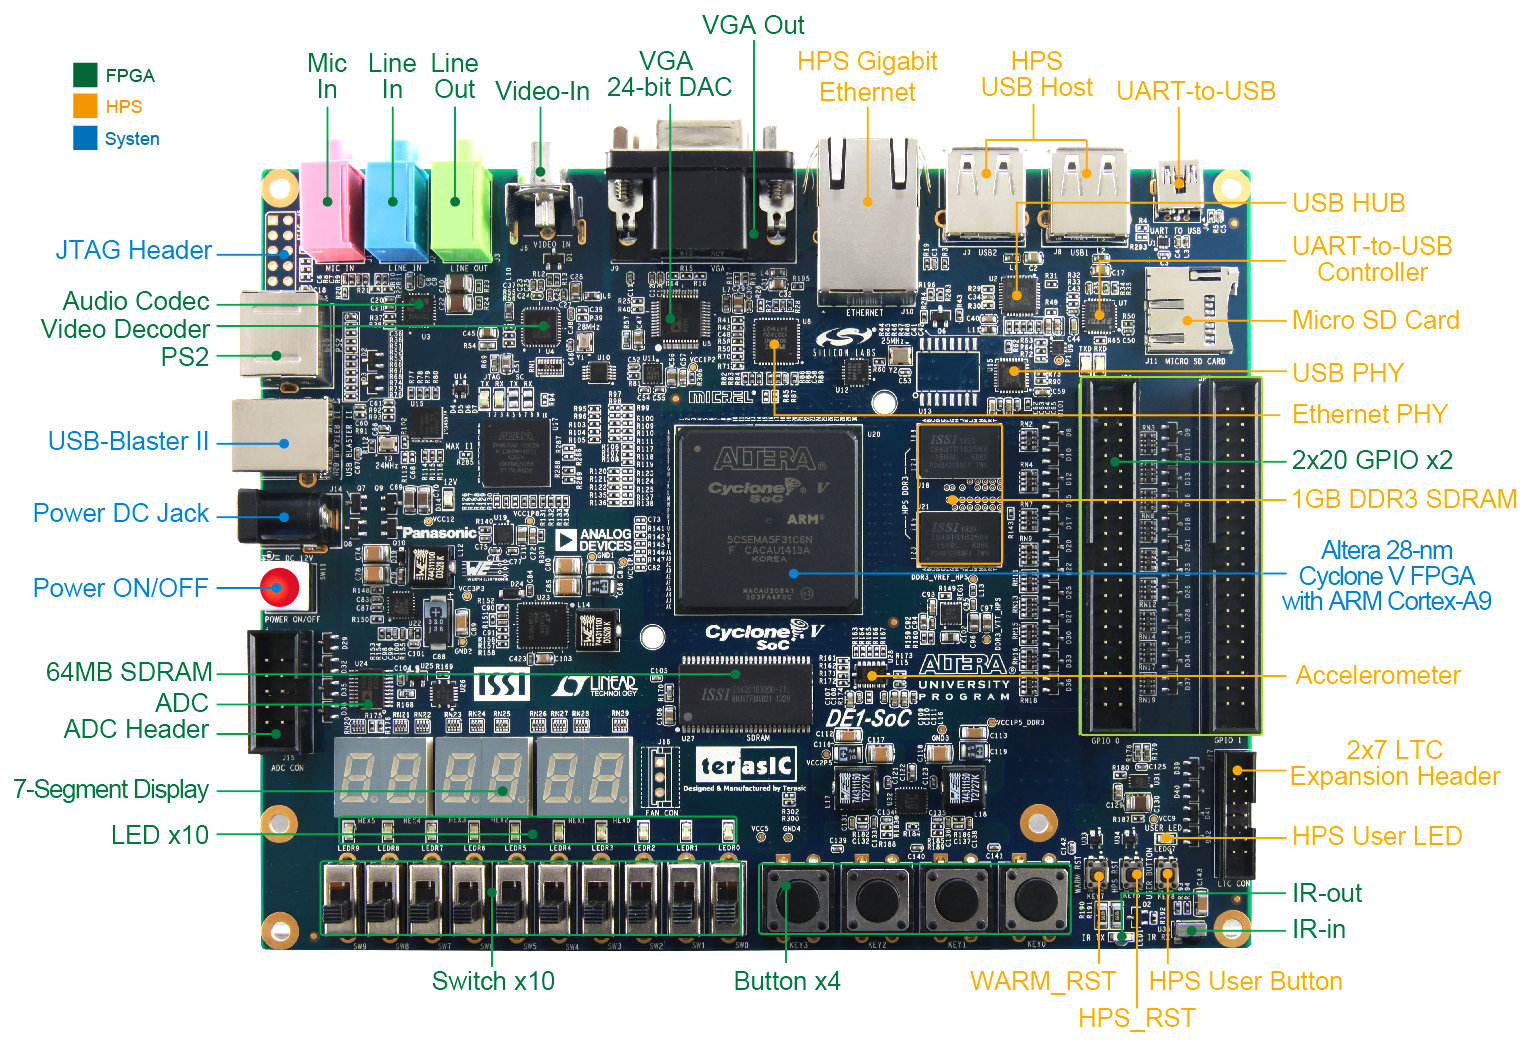
\includegraphics[width=.8\textwidth]{Figures/Board.png}
      \caption{An example showing the top layout of a DE1-SoC board}
      \label{fig:1}
    \end{figure}

  \item A VGA cable is necessary for monitor output

    \begin{figure}[h!]
      \centering
      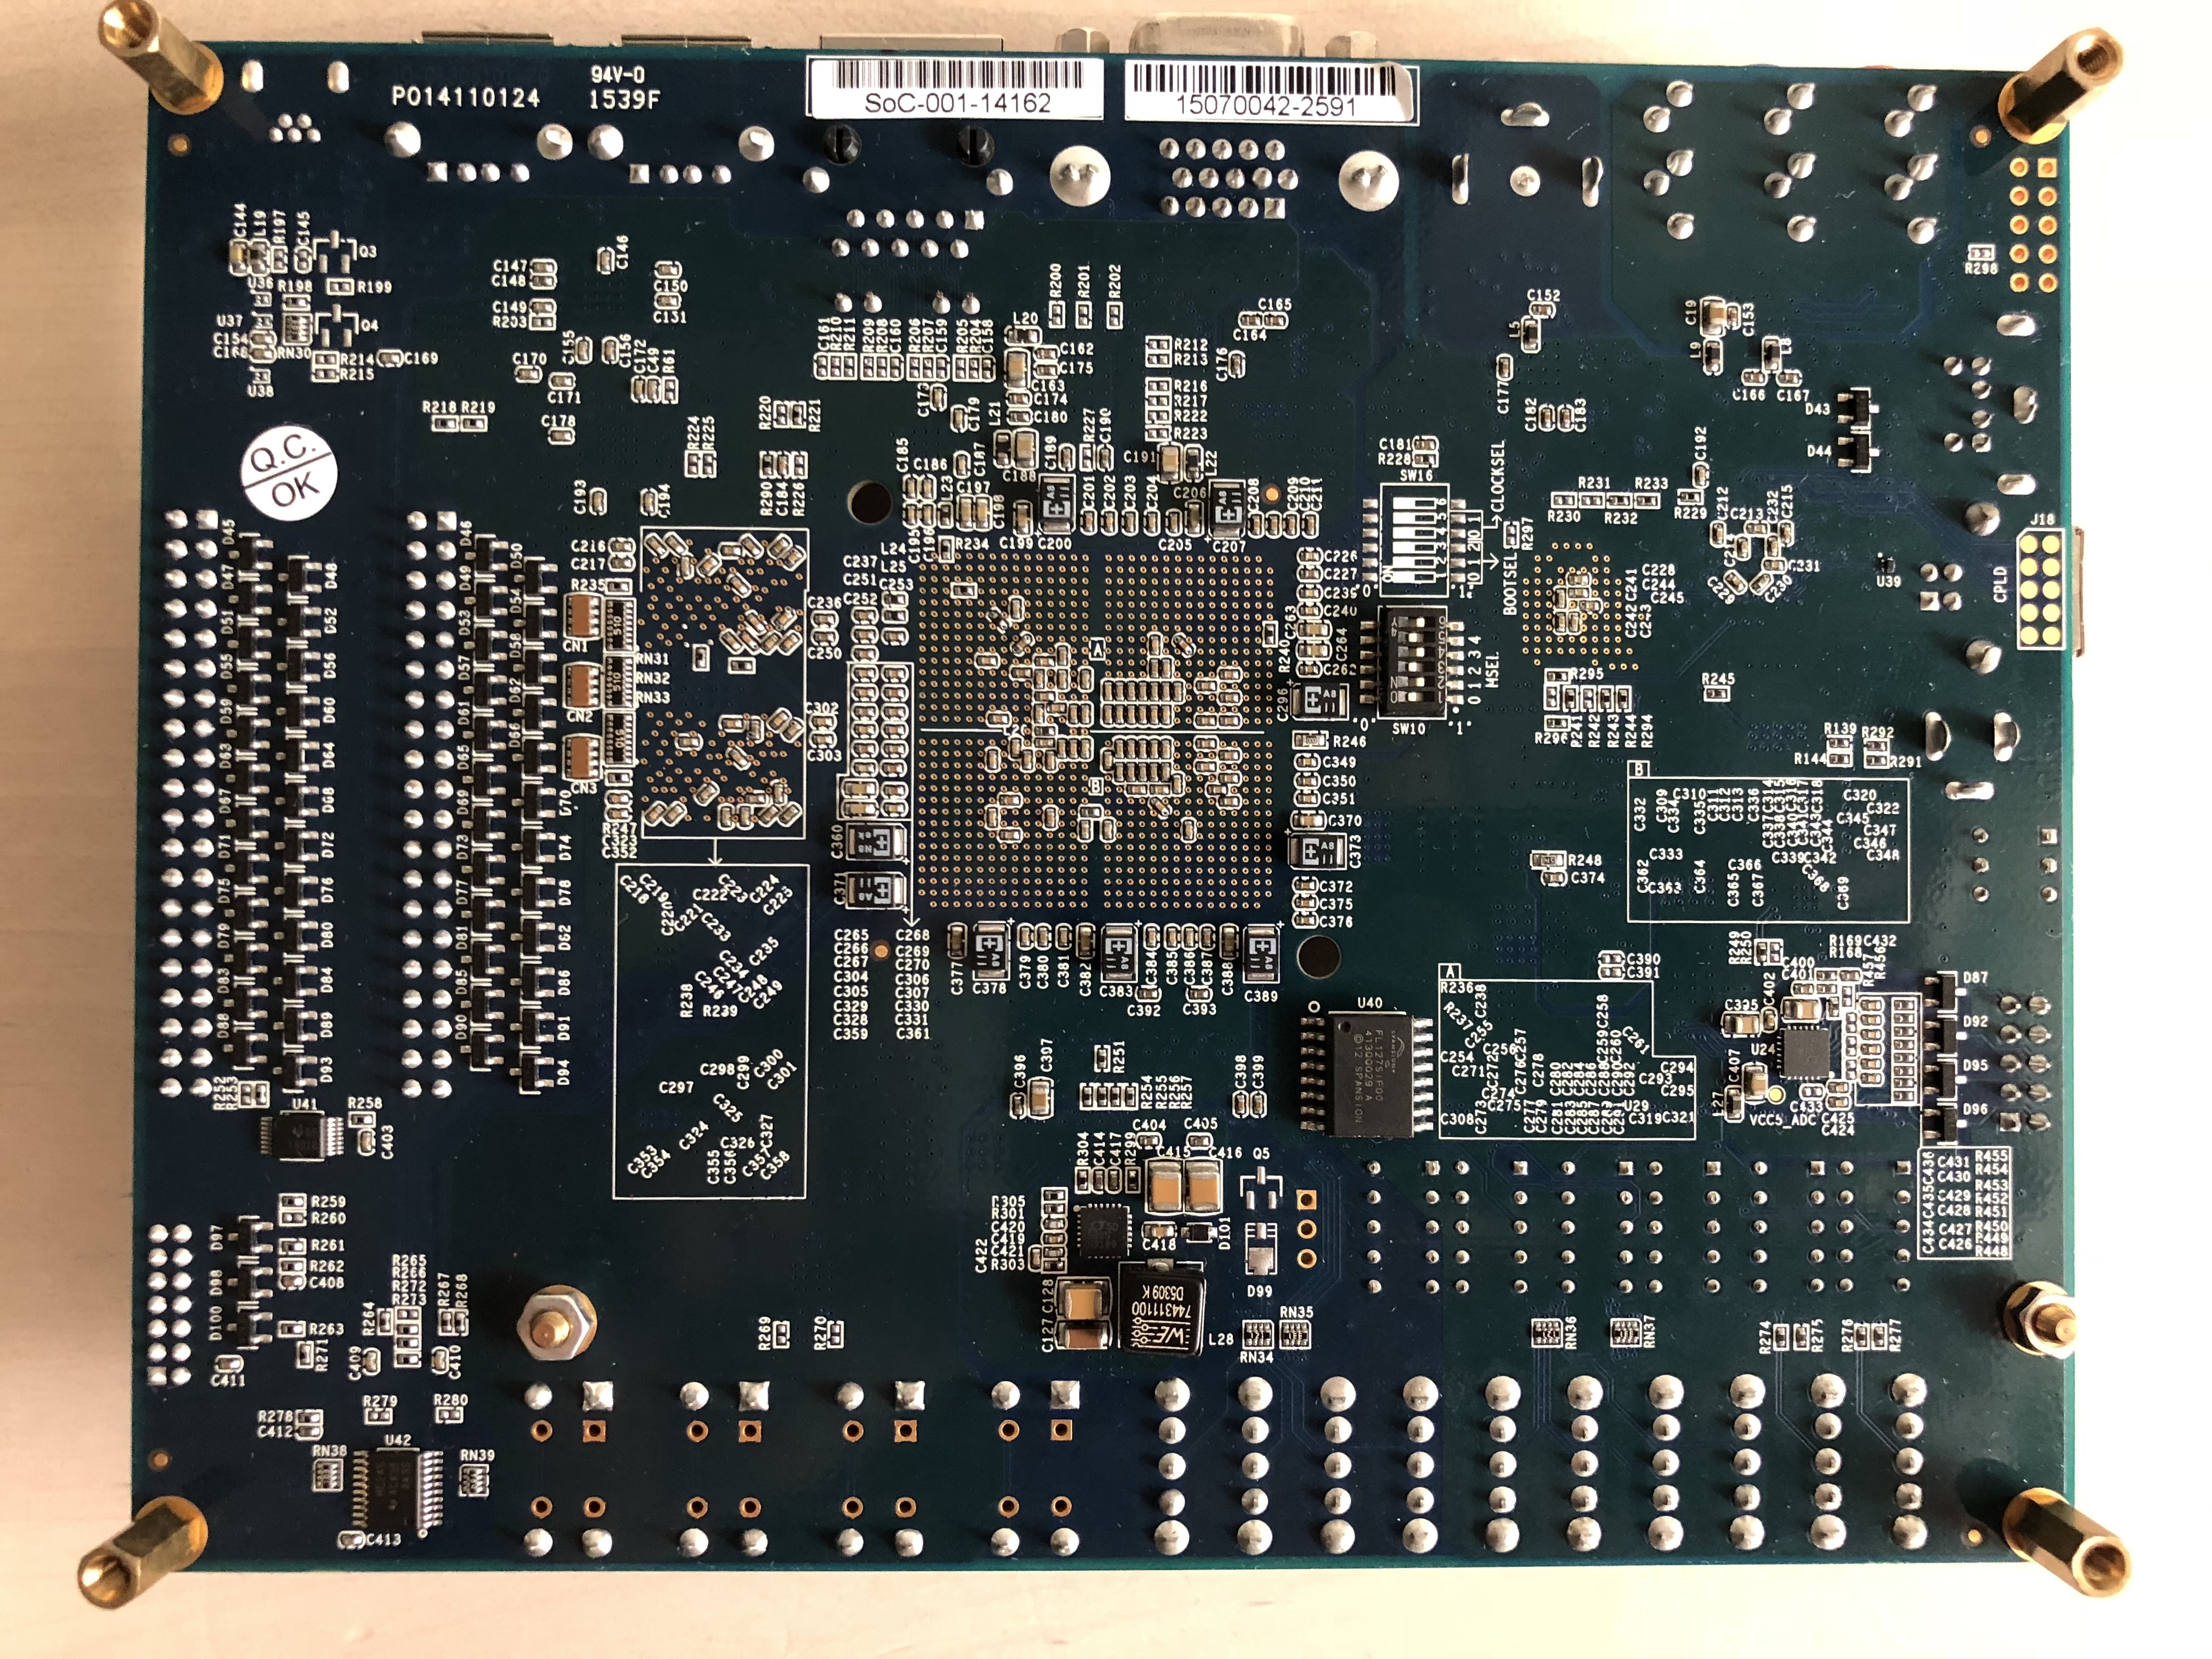
\includegraphics[width=.7\textwidth]{Figures/Board2.png}
      \caption{An example showing the bottom layout of a DE1-SoC board}
      \label{fig:2}
    \end{figure}

  \item The abstract section of the lab report should essentially be the lab introduction, but in your own words

  \item Include pictures of the board, necessary figures, and excel or MATLAB table representations of data in lab reports

  \item Conclusion sums up what was learned from the lab

  \item References are required if outside sources were used

  \item In this lab we will design a circuit capable of adding two binary numbers, and we will use the Quartus Prime Schematic to simulate and validate its behavior. This tool allows you to construct complex circuits with a hierarchical schematic design, which you can then test with different artificial inputs. We will also upload our designs into the FPGA on the Intel DE1-SoC Board and verify the designs using Switches and LEDs on the board.

  \item A half adder is a circuit capable of adding two 1-bit numbers. The circuit has two inputs and two outputs. The circuit can add two 1-bit numbers (inputs), for example, $1_2+1_2 = 10_2$. We call the least significant bit as Sum, and the most significant bit as Carry for the two outputs. 

  \item Pre-Lab Truth Table for a Half-adder Circuit:

    \begin{center}
      \begin{tabular}[h]{c c | c c}
        \textbf{A} & \textbf{B} & \textbf{Sum} & \textbf{Cout}\\
        \hline
        0 & 0 & 0 & 0\\
        0 & 1 & 1 & 0\\
        1 & 0 & 1 & 0\\
        1 & 1 & 0 & 1
      \end{tabular}
    \end{center}

  \item We will design a half-adder using Quartus Schematic and run the simulation with Waveform 

  \item Looking at the table, the circuit will have two inputs, $A$ and $B$, and two outputs, Sum and Cout

  \item Additionally, it is clear that the Carry requires an ``and'' because both $A$ and $B$ have to be 1, while Sum requires an ``xor'' because only $A$ or $B$ can be 1 to make it 1

  \item The sum can be written as Sum $=(\bar{A}\bullet B)+(A\bullet\bar{B})$

  \item The carry can be written as Cout $=A\bullet B$

  \item In this lab, we will be given the circuit drawing, but, normally, we will design the circuit ourselves

  \item The purpose of this lab is to understand how to draw a schematic and upload it to a board

  \item Once the circuit is fully designed, without error, it is necessary to test the circuit before uploading anything to the board using a simulator

    \begin{figure}[h!]
      \centering
      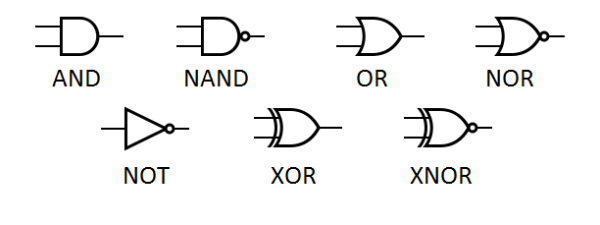
\includegraphics[width=.9\textwidth]{Figures/symbols.png}
      \caption{Logic Gate Symbols}
      \label{fig:3}
    \end{figure}

  \item We will be using the above symbols in this project

\end{itemize}

\end{document}

